\documentclass{article}
%  ╔══════════════════════════════════════════════════════════╗
%  ║                         Title                            ║
%  ╚══════════════════════════════════════════════════════════╝
%NOTE: I want \title,\author to be near top, and this \renewcommand{\maketitle} fails if these are above it.
\usepackage[utf8]{inputenc}         % Used to compile any UTF-8 Character (and supports Unicode)
\usepackage{titling}

\renewcommand{\maketitle}{
    \quad
    \vspace{1em}
  \begin{center}
      \LARGE\bfseries \thetitle \par
      \vspace{0.6em}
      \large
  \end{center}
    \vspace{1em}
}

\title{non-Hausdorfness}
\author{Nathanael Chwojko-Srawley}
\date{\today}

%  ╔══════════════════════════════════════════════════════════╗
%  ║                         packages                         ║
%  ╚══════════════════════════════════════════════════════════╝

\usepackage{extarrows}         % Used to compile any UTF-8 Character (and supports Unicode)
\usepackage{stackengine}
\usepackage{colortbl}
\usepackage{scalerel}
\usepackage{amsmath, amssymb} % Used to write better mathematical expressions (ex. \mathbb{R})
\usepackage{stackrel}         % for left-right arrows, staking symbol above and bellow
\usepackage{mathrsfs}
\usepackage{bbm}                     % for mathbbm{1}
\usepackage{euscript}
\usepackage{commutative-diagrams}
\usepackage[font=itshape]{quoting}
\usepackage{mathtools}
  \usepackage{enumitem}
\usepackage{amsthm}           % Used to create theorem enviroments.
\usepackage{graphicx}         % Let's you use images in LaTeX; ex the \includegraphics command.
\usepackage{hhline}
%\usepackage{luatexja}
%\usepackage{fontspec}
\usepackage{dsfont}
\usepackage{wasysym}          % emoji's!
\usepackage{float}            % package with ``H'' for figures and tables, ex. Images, tables, etc
%\usepackage{subcaption}      % More options with sub-captions.
\usepackage{setspace}         % More flexibility on spacing in document.
\usepackage{hyperref}         % let's me put hyperlinks
%\usepackage{tikz}             % for commutative diagrams https://tex.stackexchange.com/questions/419221/how-to-do-the-pushout-with-universal-property
\usepackage{tikz-cd}          % for commutative diagrams https://tex.stackexchange.com/questions/419221/how-to-do-the-pushout-with-universal-property
%\usepackage{quiver}           % for better commutative diagrams
\usepackage{bookmark}         % creating heading shortcut bar on the left as in word
\usepackage{longtable}        % create tables that extend past one page
%\usepackage{siunitx}         % required for alignment
%\usepackage{multirow}        % for multiple rows
\usepackage{microtype}        % makes nice text. Fixes some under-/over- filled box problems.
%\usepackage{fancyvrb}        % Let's you write code (different style than listings).
\usepackage[most]{tcolorbox} 	      % Makes nice boxes for thms, cor, prop, or anything else.
%\usepackage{enumitem}        % More flexibility on enumeration (don't know much).
\usepackage{xcolor}           % Colour text.
\usepackage{wrapfig}          % To wrap text around figure
\usepackage{listings}         % Create nice colour code blocks (customized in preamble)
\usepackage{thmtools}         % Customize theorem environment (in preamble).
%\usepackage{marvosym}        % Provide ``basic'' symbols (hazard, religious, smiley face etc.)
\usepackage{array}            % \begin{table}{>{\em}c c} -> 1st column italic (bfseries for bold)
%\usepackage[english]{babel}  % If I want to blindtext in english.
\usepackage{blindtext}
\usepackage[a4paper, total={6in, 8.5in}]{geometry}
%\usepackage[symbol]{footmisc} % For daggers and asterisk for footnotes. 1: *, 2: dagger, etc.
\usepackage{fancyhdr}
\usepackage{titlesec}
%\usepackage{pst-plot}          %To make nice plots: https://tex.stackexchange.com/questions/47594/how-can-i-make-a-graph-of-a-function#47596
% \usepackage[answerdelayed]{exercise}
\usepackage{etoolbox}          % for Dynkin diagrams
\usepackage{dynkin-diagrams}   % for Dynkin diagrams

% ╔═════════════════════════════════════════════════════╗
% ║           for figures via inkspace                  ║
% ╚═════════════════════════════════════════════════════╝

% to import figures via: https://github.com/gillescastel/inkscape-figures
\usepackage{import}
\usepackage{pdfpages}
\usepackage{transparent}


% This command is the ONLY command imported via the packages snippet, think of it as a tiny package written out
\newcommand{\incfig}[2][1]{%
    \def\svgwidth{#1\columnwidth}
    \import{./figures/}{#2.pdf_tex}
}

% ╔═══════════════════════════════════════════════════════════╗
% ║                 bibliography and citing                   ║
% ╚═══════════════════════════════════════════════════════════╝
% \usepackage[backend=biber,citestyle=alphabetic,bibstyle=authortitle]{biblatex}

\usepackage{csquotes}
\usepackage{biblatex}

\addbibresource{bibliography.bib}

% ╔═══════════════════════════════════════════════════════════╗
% ║                    colours (colors)                       ║
% ╚═══════════════════════════════════════════════════════════╝

\definecolor{dkgreen}{rgb}{0,0.6,0}
\definecolor{gray}{rgb}{0.5,0.5,0.5}
\definecolor{mauve}{rgb}{0.58,0,0.82}
\definecolor{lightyellow}{rgb}{1,1,0.6}
\definecolor{reddish}{HTML}{A01A3A}

%  ╔══════════════════════════════════════════════════════════╗
%  ║                       book format                        ║
%  ╚══════════════════════════════════════════════════════════╝

\pagestyle{fancy}

\setlength\headheight{20pt}

\renewcommand{\sectionmark}[1]{\markright{\thesection.\ #1}}

\fancyfoot[C,CO]{\textcolor{gray}{Nathanael Chwojko-Srawley}}
\fancyfoot[R,RO]{\thepage}{}

% Create a new page style for the first page
\fancypagestyle{firstpage}{
  \fancyhf{} % Clear header and footer
  \fancyhead[L]{\theauthor}
  \fancyhead[R]{\today} % Date in the top-right
  \fancyfoot[C]{\textcolor{gray}{Nathanael Chwojko-Srawley}}
  \fancyfoot[R]{\thepage}
}

% Apply the first page style conditionally
\AtBeginDocument{\thispagestyle{firstpage}}

%have format the title command
\newcommand{\chapter}[1]{%
  \clearpage
  \vspace*{30pt} % Space before the chapter title
  {\normalfont\huge\bfseries #1\par} % Chapter title formatting
  \vspace{20pt} % Space after the chapter title
}


\setlength{\parindent}{0pt} % don't like indentation infront of paragraphs
\setlength{\parskip}{1ex}   %so that there is still space between paragarphs


%  ╔══════════════════════════════════════════════════════════╗
%  ║                       Shortcuts                          ║
%  ╚══════════════════════════════════════════════════════════╝

%\ExerciseLevelInToc

% I like original mathcal better, but need lowercase.
\DeclareFontFamily{OT1}{pzc}{}
\DeclareFontShape{OT1}{pzc}{m}{it}{<-> s * [1.10] pzcmi7t}{}
\DeclareMathAlphabet{\mathpzc}{OT1}{pzc}{m}{it}


% mathbb
\newcommand{\A}{{\mathbb{A}}}
\newcommand{\C}{{\mathbb{C}}}
\newcommand{\F}{{\mathbb{F}}}
\newcommand{\N}{{\mathbb{N}}}
\newcommand{\Q}{{\mathbb{Q}}}
\newcommand{\R}{{\mathbb{R}}}
\newcommand{\V}{{\mathbb{V}}}
\newcommand{\Z}{{\mathbb{Z}}}
\newcommand{\BI}{{\mathbb{I}}}
\renewcommand{\H}{{\mathbb{H}}}
\renewcommand{\P}{{\mathbb{P}}}


% mathcal
% \newcommand{\co}{{\mathfrak{o}}} %mathcal{o} looks like wreath product, so I changed it to mathfrak
\newcommand{\co}{{\mathpzc{o}}}
\newcommand{\CA}{{\mathcal{A}}}
\newcommand{\CB}{{\mathcal{B}}}
\newcommand{\CC}{{\mathcal{C}}}
\newcommand{\CD}{{\mathcal{D}}}
\newcommand{\CF}{{\mathcal{F}}}
\newcommand{\CG}{{\mathcal{G}}}
\newcommand{\CH}{{\mathcal{H}}}
\newcommand{\CI}{{\mathcal{I}}}
\newcommand{\CK}{{\mathcal{K}}}
\newcommand{\CL}{{\mathcal{L}}}
\newcommand{\CM}{{\mathcal{M}}}
\newcommand{\CN}{{\mathcal{N}}}
\newcommand{\CO}{{\mathcal{O}}}
\newcommand{\CQ}{{\mathcal{Q}}}
\newcommand{\CR}{{\mathcal{R}}}
\newcommand{\CS}{{\mathcal{S}}}
\newcommand{\CT}{{\mathcal{T}}}
\newcommand{\CV}{{\mathcal{V}}}
\newcommand{\CZ}{{\mathcal{Z}}}
% EXCPETION:
\newcommand{\CP}{{\mathcal{P}}}
% \newcommand{\CP}{\mathbb{C}\mathrm{P}}
\newcommand{\RP}{\mathbb{R}\mathrm{P}}


%Euscript
\newcommand{\EB}{\EuScript{B}}
\newcommand{\EC}{{\EuScript{C}}}
\newcommand{\EF}{{\EuScript{F}}}
\newcommand{\EL}{{\EuScript{L}}}
\newcommand{\EO}{{\EuScript{O}}}


%mathfrak (lowercase)
\newcommand{\fa}{{\mathfrak{a}}}
\newcommand{\fb}{{\mathfrak{b}}}
\newcommand{\fc}{{\mathfrak{c}}}
\newcommand{\fd}{{\mathfrak{d}}}
\newcommand{\fm}{{\mathfrak{m}}}
\newcommand{\fn}{{\mathfrak{n}}}
\newcommand{\fo}{{\mathfrak{o}}}
\newcommand{\fp}{{\mathfrak{p}}}
\newcommand{\fq}{{\mathfrak{q}}}


%mathfrak (upper case)
\newcommand{\FA}{{\mathfrak{A}}}
\newcommand{\FB}{{\mathfrak{B}}}
\newcommand{\FC}{{\mathfrak{C}}}
\newcommand{\FD}{{\mathfrak{D}}}
\newcommand{\FK}{{\mathfrak{K}}}
\newcommand{\FM}{{\mathfrak{M}}}
\newcommand{\FN}{{\mathfrak{N}}}
\newcommand{\FO}{{\mathfrak{O}}}
\newcommand{\FP}{{\mathfrak{P}}}


%mathscr
\newcommand{\ff}{{\mathscr{F}}}
\newcommand{\SA}{\mathscr{A}}
\newcommand{\SC}{\mathscr{C}}
\newcommand{\SF}{\mathscr{F}}
\newcommand{\SG}{\mathscr{G}}
\newcommand{\SH}{\mathscr{H}}
\newcommand{\SI}{\mathscr{I}}
\newcommand{\SK}{\mathscr{K}}
\newcommand{\SN}{\mathscr{N}}
\newcommand{\SQ}{\mathscr{Q}}
\newcommand{\SR}{\mathscr{R}}
\newcommand{\SV}{\mathscr{V}}
\newcommand{\SZ}{\mathscr{Z}}


% operatorname -- 2 letters (lowercase and upper case)
\newcommand{\ab}{{\operatorname{ab}}}
\newcommand{\ad}{{\operatorname{ad}}}
\newcommand{\ch}{{\operatorname{ch}}}
\newcommand{\ev}{{\operatorname{ev}}}
\newcommand{\id}{{\operatorname{id}}}
\newcommand{\im}{{\operatorname{im}}}
\newcommand{\nm}{{\operatorname{Nm}}}
\newcommand{\op}{{\operatorname{op}}}
\newcommand{\rk}{{\operatorname{rk}}}
\newcommand{\sh}{{\operatorname{sh}}}
\newcommand{\tr}{{\operatorname{tr}}}

\newcommand{\Ab}{{\operatorname{Ab}}}
\newcommand{\Br}{{\operatorname{Br}}}
\newcommand{\Ch}{{\operatorname{Ch}}}
\newcommand{\Cl}{{\operatorname{Cl}}}
\newcommand{\GL}{{\operatorname{GL}}}
\newcommand{\Nm}{{\operatorname{Nm}}}
\newcommand{\SL}{{\operatorname{SL}}}

\renewcommand{\Re}{{\operatorname{Re}}}
\renewcommand{\Im}{{\operatorname{Im}}}


%categories
\newcommand{\Grp}{{\textbf{Grp}}}
\newcommand{\Fld}{{\textbf{Fld}}}
\newcommand{\Sh}{{\textbf{Sh}}}
\newcommand{\Set}{{\textbf{Set}}}
\newcommand{\Mod}{{\textbf{Mod}}}
\newcommand{\PSh}{{\textbf{PSh}}}
\newcommand{\Sch}{{\textbf{Sch}}}
\newcommand{\Top}{{\textbf{Top}}}
\newcommand{\RgSp}{{\textbf{RgSp}}}
\newcommand{\Ring}{{\textbf{Ring}}}


%operatorname -- 3+ letters (lowercase and upper case)
\newcommand{\rad}{{\operatorname{rad}}}
\newcommand{\sep}{{\operatorname{sep}}}
\newcommand{\res}{{\operatorname{res}}}
\newcommand{\sgn}{{\operatorname{sgn}}}
\newcommand{\pre}{{\operatorname{pre}}}
\newcommand{\ord}{{\operatorname{ord}}}
\newcommand{\vol}{{\operatorname{vol}}}
\newcommand{\lcm}{{\operatorname{lcm}}}

\newcommand{\conj}{{\operatorname{conj}}}
\newcommand{\disc}{{\operatorname{disc}}}
\newcommand{\stab}{{\operatorname{stab}}}
\newcommand{\kdim}{{\operatorname{kdim}}}
\newcommand{\diag}{{\operatorname{diag}}}

\newcommand{\trdeg}{\operatorname{trdeg}}
\newcommand{\coker}{{\operatorname{coker}}}
\newcommand{\codim}{{\operatorname{codim}}}

\newcommand{\Ann}{{\operatorname{Ann}}}
\newcommand{\Aut}{{\operatorname{Aut}}}
\newcommand{\Der}{{\operatorname{Der}}}
\newcommand{\Div}{{\operatorname{Div}}}
\newcommand{\Emb}{{\operatorname{Emb}}}
\newcommand{\End}{{\operatorname{End}}}
\newcommand{\Ext}{{\operatorname{Ext}}}
\newcommand{\Gal}{{\operatorname{Gal}}}
\newcommand{\Hom}{{\operatorname{Hom}}}
\newcommand{\Ind}{{\operatorname{Ind}}}
\newcommand{\Inn}{{\operatorname{Inn}}}
\newcommand{\Int}{{\operatorname{int}}}
\newcommand{\Irr}{{\operatorname{Irr}}}
\newcommand{\Jac}{{\operatorname{Jac}}}
\newcommand{\Mor}[1]{\operatorname{Mor}(\textbf{#1})}
\newcommand{\Nil}{{\operatorname{Nil}}}
\newcommand{\Obj}{{\operatorname{Obj}}}
\newcommand{\Out}{{\operatorname{Out}}}
\newcommand{\Pic}{{\operatorname{Pic}\,}}
\newcommand{\Rep}{{\operatorname{Rep}}}
\newcommand{\Res}{{\operatorname{Res}}}
\newcommand{\Spl}{{\operatorname{Spl}}}
\newcommand{\Syl}{{\operatorname{Syl}}}
\newcommand{\Sym}{{\operatorname{Sym}}}
\newcommand{\Tor}{{\operatorname{Tor}}}

\newcommand{\Char}{{\operatorname{char}}}
\newcommand{\Frac}{{\operatorname{Frac}}}
\newcommand{\Frob}{{\operatorname{Frob}}}
\newcommand{\Proj}{{\operatorname{Proj}\,}}
\newcommand{\RMod}{{}_R\operatorname{Mod}}
\newcommand{\SExt}{{\mathcal{E}\emph{xt}}}
\newcommand{\SHom}{{\emph{Hom}}}
\newcommand{\Span}{{\operatorname{span}}}
\newcommand{\Spec}{{\operatorname{Spec}\,}}
\newcommand{\Supp}{{\operatorname{Supp}}}
\newcommand{\Tens}[1]{#1\otimes --}
\newcommand{\fHom}[1]{\operatorname{Hom}(#1, --)}

\newcommand{\mSpec}{{\operatorname{mSpec}}}
\newcommand{\cofHom}[1]{\operatorname{Hom}(--, #1)}


% connectors
% \renewcommand{\mid}{\big|}
\newcommand{\sse}{\subseteq}
\newcommand{\subg}{\leqslant}
\newcommand{\supg}{\geqslant}
\newcommand{\ssne}{\subsetneq}
\newcommand{\isosubg}{\lesssim}
\newcommand{\nsse}{\not\subseteq}
\newcommand{\nsubg}{\trianglelefteq}
\newcommand{\nsupg}{\trianglerighteq}
\newcommand{\csubg}{\blacktriangleleft}
\renewcommand{\mid}{\big|}


% Arrows
\newcommand{\rw}{\rightarrow}
\newcommand{\Rw}{\Rightarrow}
\newcommand{\lw}{\leftarrow}
\newcommand{\Lw}{\Leftarrow}
\newcommand{\lrw}{\leftrightarrow}
\newcommand{\LRw}{\Leftrightarrow}
\newcommand{\acton}{\curvearrowright}
\newcommand{\actson}{\curvearrowright}
\newcommand\mapsfrom{\mathrel{\reflectbox{\ensuremath{\mapsto}}}}

% arrows for commutative diagram: create four new angled double-struck arrows
\newcommand\myrot[1]{\mathrel{\rotatebox[origin=c]{#1}{$\Rightarrow$}}}
\newcommand\NEarrow{\myrot{45}}
\newcommand\NWarrow{\myrot{135}}
\newcommand\SWarrow{\myrot{-135}}
\newcommand\SEarrow{\myrot{-45}}


%shorthands
\newcommand{\oln}[1]{{\overline{#1}}}
\renewcommand{\bf}[1]{\textbf{#1}}
\newcommand{\qn}{\quad\newline}


% limits
\newcommand{\Lim}{{\varprojlim}}
\newcommand{\coLim}{{\varinjlim}}
\newcommand{\Dlim}{\lim\limits_{\longrightarrow}}
\newcommand{\coDlim}{\lim\limits_{\longleftarrow}}


%for saturated ideals in the localization section (I don't like these, I think I'll delete)
\newcommand{\LIm}{{}^e }
\newcommand{\LPre}{{}^c }

%  ╔══════════════════════════════════════════════════════════╗
%  ║                    Custom Commands                       ║
%  ╚══════════════════════════════════════════════════════════╝

% swap varphi and phi
\let\temp\phi
\let\phi\varphi
\let\varphi\temp

\newcommand{\placeholder}{\_\_\_\_\_}

\newcommand{\set}[2]{\left\{#1 \ \middle|\ #2\right\}}

%mod should not have the crazy amount of space to its right!
\renewcommand{\mod}{\,\operatorname{mod}\,}

% dcups
\newcommand{\dcup}{\sqcup}
\newcommand{\Dcup}{\coprod}
% \newcommand{\Dcup}{\bigsqcup}

\newcommand{\nbot}{\mathrel{\rlap{$\bot$}\mkern2mu/}}

%a nice large circle
\newcommand{\tikzcircle}[2][red,fill=black]{\tikz[baseline=-0.5ex]\draw[#1,radius=#2] (0,0) circle ;}%

\makeatletter
\newcommand*\bigcdot{\mathpalette\bigcdot@{.5}}
\newcommand*\bigcdot@[2]{\mathbin{\vcenter{\hbox{\scalebox{#2}{$\m@th#1\bullet$}}}}}
\makeatother

%somehow not a default command
\def\rddots{\mathstrut^{.^{.^{.}}}}

%% new delimiter
\DeclarePairedDelimiter{\ceil}{\lceil}{\rceil}


%  ╔══════════════════════════════════════════════════════════╗
%  ║                     environments                         ║
%  ╚══════════════════════════════════════════════════════════╝


%remember the option: breakable

% create tcolor boxes
\newtcbtheorem[number within=section]{thm}{Theorem}%
{
colback=green!5,
colframe=green!35!black,
fonttitle=\bfseries,
label type=theorem
}{th}

\newtcbtheorem[number within=section, use counter from=thm]{lem}{Lemma}%
{
colback=blue!5,
colframe=black!35!black,
fonttitle=\bfseries,
label type=lemma
}{lm}
\newtcbtheorem[number within=section, use counter from=thm]{prop}{Proposition}%
{
colback=white!5,
colframe=white!35!black,
fonttitle=\bfseries,
label type=proposition
}{pr}
\newtcbtheorem[number within=section, use counter from=thm]{cor}{Corollary}%
{colback=blue!5,
colframe=blue!35!black,
fonttitle=\bfseries,
label type=corollary
}{co}
\newtcbtheorem[number within=section, use counter from=thm]{axiom}{Axiom}%
{colback=black!5,
colframe=yellow!35!black,
fonttitle=\bfseries,
label type=axiom
}{ax}
\newtcbtheorem[number within=section, use counter from=thm]{defn}{Definition}%
{colback=red!5,
colframe=red!35!black,
fonttitle=\bfseries,
label type=definition
}{df}


% for <s-cr> to create \item[$\LRw$] instead of \item
\newenvironment{equivEnumerate}
 {\begin{enumerate}
	}{
\end{enumerate}}



%Custom enviroments
 \newenvironment{note}
 {\begin{tcolorbox}[enhanced, sharp corners, colback=white , borderline={0.2pt}{0pt}{black}]
   \begin{quote}\textbf{Note}:
   }{
   \end{quote}\end{tcolorbox}}

 \newenvironment{intuition}
 {\begin{quote}\textbf{Intuition}:
   }{
   \end{quote}}

\newtcbtheorem[number within=section, use counter from=thm]{titledBox}{}{%
  enhanced,
  sharp corners,
  colback=white,
  colframe=black,
  borderline={0.2pt}{0pt}{black},
  left=2mm,
  right=2mm,
  top=2mm,
  bottom=2mm,
  title style={opacity=1},
  attach title to upper,
  before upper={\textbf{\tcbtitletext}\quad},
  coltitle=black,
  fonttitle=\bfseries,
  separator sign={\quad}
}{box}


%better example and proof environments
\def\exampletext{Example} % If English
\colorlet{colexam}{red!55!black} % Global example color


\newtcbtheorem[number within=section, use counter from=thm]{example}{Example}{% \newtcolorbox[use counter=testexample]{testexamplebox}{%
% Example Frame Start
empty,% Empty previously set parameters
title={\exampletext \thetcbcounter #1},% use \thetcbcounter to access the testexample counter text
% Attaching a box requires an overlay
attach boxed title to top left,
   % Ensures proper line breaking in longer titles
   minipage boxed title,
% (boxed title style requires an overlay)
boxed title style={empty,size=minimal,toprule=0pt,top=4pt,left=3mm,overlay={}},
coltitle=colexam,fonttitle=\bfseries,
before=\par\medskip\noindent,parbox=false,boxsep=0pt,left=3mm,right=0mm,top=2pt,breakable,pad at break=0mm,
   before upper=\csname @totalleftmargin\endcsname0pt, % Use instead of parbox=true. This ensures parskip is inherited by box.
% Handles box when it exists on one page only
overlay unbroken={\draw[colexam,line width=.5pt] ([xshift=-0pt]title.north west) -- ([xshift=-0pt]frame.south west); },
% Handles multipage box: first page
overlay first={\draw[colexam,line width=.5pt] ([xshift=-0pt]title.north west) -- ([xshift=-0pt]frame.south west); },
% Handles multipage box: middle page
overlay middle={\draw[colexam,line width=.5pt] ([xshift=-0pt]frame.north west) -- ([xshift=-0pt]frame.south west); },
% Handles multipage box: last page
overlay last={\draw[colexam,line width=.5pt] ([xshift=-0pt]frame.north west) -- ([xshift=-0pt]frame.south west); }%
}{ex}



\def\prooftext{Proof} % If English
\NewDocumentEnvironment{Proof}{ O{} }
{
    \colorlet{colexam}{black!55!black} % Global example color
    \newtcolorbox[number within=section]{testproofbox}{%
        empty,% Empty previously set parameters
        title={\emph{\prooftext} \thetcbcounter: #1},
        attach boxed title to top left,
        minipage boxed title,
        boxed title style={empty,size=minimal,toprule=0pt,top=4pt,left=3mm,overlay={}},
        coltitle=colexam,
        fonttitle=\bfseries,
        before=\par\medskip\noindent,
        parbox=false,
        boxsep=0pt,
        left=3mm,
        right=0mm,
        top=2pt,
        breakable,
        pad at break=0mm,
        before upper=\csname @totalleftmargin\endcsname0pt,
        % Removed height constraints
        % Added flexible width
        width=\dimexpr\textwidth-3mm\relax,
        % Modified overlays
        overlay unbroken={\draw[colexam,line width=.5pt] ([xshift=-0pt]title.north west) -- ([xshift=-0pt]frame.south west); },
        overlay first={\draw[colexam,line width=.5pt] ([xshift=-0pt]title.north west) -- ([xshift=-0pt]frame.south west); },
        overlay middle={\draw[colexam,line width=.5pt] ([xshift=-0pt]frame.north west) -- ([xshift=-0pt]frame.south west); },
        overlay last={\draw[colexam,line width=.5pt] ([xshift=-0pt]frame.north west) -- ([xshift=-0pt]frame.south west); },%
    }
    \begin{testproofbox}
}
{\end{testproofbox}\endlist}


%  ╔══════════════════════════════════════════════════════════╗
%  ║                    for Dynkin diagrams                   ║
%  ╚══════════════════════════════════════════════════════════╝

\def\row#1/#2!{#1_{\IfStrEq{#2}{}{n}{#2}} & \dynkin{#1}{#2}\\}
\newcommand{\tble}[1]{
   \renewcommand*\do[1]{\row##1!}
   \[
      \begin{array}{ll}\docsvlist{#1}\end{array}
   \]
}

%  ╔══════════════════════════════════════════════════════════╗
%  ║                         links                            ║
%  ╚══════════════════════════════════════════════════════════╝

\definecolor{LinkColour}{HTML}{A64A3B} % favourite
% \definecolor{LinkColour}{HTML}{8C3D32} % 2nd place
\hypersetup{
  colorlinks,
  citecolor=black,
  filecolor=magenta,
  linkcolor=LinkColour,
  urlcolor=blue,
}


%  ╔══════════════════════════════════════════════════════════╗
%  ║                          misc                            ║
%  ╚══════════════════════════════════════════════════════════╝

\stackMath %to be able to stack text in math mode
\makeindex

%import options: all, bibliography, book-formatting, booksSetting, customEnvironments, dynkin, hw-formatting, language-setup, newcommands, packages, preamble, proofs, settings, tcolorbox, test.svg,
\begin{document}
\maketitle

This is a short blog to explain and construct a non-Hausdorff spaces to someone with no university background
in mathematics. In one sentence
\begin{center}
  \emph{A non-Hausdorff space is a space where points can be infinitely close to each other without being the
  same point}
\end{center}
Hausdorffness is a concept that is usually introduced in a class in topology and relies on many little ideas that
naturally show the necessity for defining Hausdorffness. These ideas are presented here with as little mathematical
build-up as possible, but as a consequence it is likely the reader will have to spend some time digesting the
concepts.

In this blog, there shall be some apocrypha's for the sake of not overloading on technicalities, and these shall be
sorted in an extra section for those with the appropriate topological background.


\section{Build up}

The set of all numbers that are not complex are called the \emph{real number line} and is denoted $\R$. It is
often drawn as:
\[
\begin{tikzpicture}
  \draw[thick] (-3,1) -- (3,1) node[left=7cm] {$\R$};
  \foreach \x in {-3,-2,-1,0,1,2,3} {
    \draw[thick] (\x,0.9) -- (\x,1.1);
    \node[below] at (\x,0.8) {$\x$};
  }
  \node[left] at (-3,1) {$\cdots$};
  \node[right] at (3,1) {$\cdots$};
\end{tikzpicture}
\]
An element of $\R$ is called a \emph{real number} (to distinguish from complex
numbers). Let us choose any two real numbers, say $3$ and $4$. Then they are a distance $1$ apart from each
other. Any two \emph{distinct} real numbers $x,y$ have some distance, namely $x-y$ or $y-x$ (depending on
which number is bigger). If the distance distance between two real numbers is $0$, then they are the same
number, since:
\[
  x-y = 0 \qquad \text{then} \qquad x = y
\]
But there are spaces in which you can have two points that have \emph{zero distance} between them and yet are
\emph{distinct}! It was a mathematician named Felix Hausdorff that first stumbled upon such a weird space,
and wanted to make it clear when working with a space where distinct points cannot have 0 distance from each
other. In his honour, a space in which there can't exist distinct points that have zero distance are called
\emph{Hausdorff spaces}, and the weird spaces are called \emph{non-Hausdorff} otherwise. For example the real
numbers $\R$ is Hausdorff.

\section{What is a Space?}

What is meant here by ``space''? The first encounter we all have with the notion of ``space'' is within the
world we live in: we consider the ``space'' of a room, or the routes of a hiking trail the ``space'' on which
we can walk. These two examples of spaces are very different from each other (in a room, we have 3 directions,
while for hiking trails we usually are limited to lines to follow), and there are many more such examples that
come up in the sciences (for example, we consider all possible outputs of a experiment the ``total space'' of
outcomes). This generality of the notion of space has lead mathematics to define the notion of \emph{topology}
which is a vast generalization of the Cartesian plane. Going through the technicalities of defining a topology
would distract from the specific goal of constructing a non-Hausdorff space. In fact, defining spaces in
higher than $1$ dimension would increase the technicalities, and so we shall stick to $1$-dimensions.
Thus, for our purposes, we shall define a (1-dimensional) space
as:

\begin{quote}
  \emph{A space is a set that:}
\begin{itemize}
  \item \emph{contains numbers and}
  \item \emph{possibly contains sets of numbers}
\end{itemize}
\end{quote}
% Thus we
% will construct a $1$-dimensional space that is not Hausdorff.
This is very abstract, so let us immediately justify this definition. Let us start by being precise what we
mean by \emph{set}. A set is simply the way mathematicians group things, for example here are two
different sets, one containing the numbers $1,2,3$ and the other the numbers $3,4,5$:
\[
  \{1,2,3\} \qquad \text{and} \qquad \{3,4,5\}
\]
where we used the $\{, \}$ notation to enclose the elements we are considering. Sets can hold objects other
than numbers, for an arbitrary example a set can contain all the words in the English dictionary:
\[
  S = \{\text{..., Hamiltonian, characteristic, Hypothesis, ...}\}
\]
A set can also contain other sets (think by analogy a warehouse that has boxes containing stuff):
\[
  W = \{\{\text{Alice in Wonderland, Introduction to Analysis}\}, \{\text{spoon, fork, knife}\}\}
\]

A space will be a set that contains numbers and potentially sets of numbers
\[
  R = \{1,2,\{3,4\}\}
\]
Let us justify why such a set can be thought of as a space. The simplest space is $\R$ which is the set of all
numbers and geometrically is thought of as a line. To recover lines of finite length, we can take all the
points that lie between two points, for example:
\[
  [0,1] = \{\text{$x$ in $\R$ such that $0\le x \le 1$}\}
\]
which we can visualize as:
\[
\begin{tikzpicture}
  \draw[thick] (0,0) -- (1,0);
  \draw[black, fill=black] (0,0) circle (0.1) node[below] {0};
  \draw[black, fill=black] (1,0) circle (0.1) node[below] {1};
\end{tikzpicture}
\]
This is an infinite set as it contains all numbers between $0$ and $1$ (including $0$ and $1$). We can also
take a finite subset, for example $\{1,2,3\}$ is three numbers from $\R$ and can be represented as three points:
\[

\begin{tikzpicture}
  \foreach \x in {1,2,3} {
    \fill[black] (\x,0) circle (0.1);
    \node[below] at (\x,-0.3) {\x};
  }
\end{tikzpicture}
\]
We can also take all points that lie \emph{strictly} between two points, for example:
\[
  (0,1) = \{\text{$x$ in $\R$ such that $0< x < 1$}\}
\]
Notice that $0$ is not in $(0,1)$ because $0$ is strictly smaller, $<$, than any point in $(0,1)$, and
similarly for $1$. Such examples of spaces fall under the first case of the definition ``a set
containing numbers''. Let us now justify the 2nd part of the definition: ``possibly containing sets of
numbers''. The idea is that the numbers should be considered as points, and the sets of numbers should be
thought of as being points that are \emph{glued together}.

\subsubsection*{Principle of Gluing}

Let us demonstrate this with an example: the following set splits the even and the odd
numbers into two sets:
\[
  P = \{\{0,2,4,6,...\}, \{1,3,5,7,...\}\} = \{E, O\}
\]
where we labeled the sets within $P$
\begin{itemize}
  \item $E$ for even numbers, and
  \item $O$ for odd numbers
\end{itemize}
Notice that $P$ only has \emph{two} sets (each set contains infinitely elements), and hence $P$ only contains
$2$ points. The way to think about these points is to interpret all the elements within $E$ being ``equal''
(or glued) to each other and similarly all the elements within $O$ being ``equal'' (or glued) to each other.
In mathematical notation:
\[
  0 = 2 = 4 = \cdots \qquad \text{and} \qquad 1 = 3 = 5 = \cdots \qquad \text{but} \qquad 0 \ne 1,\ 4\ne 7,\
  \text{etc.}
\]
We can think of the twos sets of $P$ as \emph{only} remembering the \emph{parity} of each number. It
does not care if a number is bigger or smaller or divisible by $5$, it only cares if it is even or odd. The
equality in the above equation is an \emph{equality of parity}, meaning two numbers are the same if they have
the same parity. Using the equal sign ``$=$'' is confusing as we already use it to mean to numbers are
``exactly equal'' not just ``equal in parity'' (or as a mathematician would say, equal \emph{up to parity}).
Let us thus create a new symbol $\sim_P$ and write:
\[
  \ 0\  \sim_P \ 2\  \sim_P \ 4\  \sim_P \cdots \qquad \text{and} \qquad \ 1\  \sim_P \ 3\  \sim_P \ 5\  \sim_P \cdots
\]
So $a\ \sim_P\ b$ is both $a$ and $b$ are even, or both $a$ and $b$ are odd, and otherwise we write $a\
\not\sim_P\ b$. Geometrically, we say that we \emph{glued} these points together. If we consider
the natural numbers $\{0,1,2,..\}$ as a space, it would be infinitely many points like so:
\[

\begin{tikzpicture}
  \foreach \x in {0,1,2,3,4,5,6,7,8,9} {
    \fill[black] (\x,0) circle (0.1);
    \node[below] at (\x,-0.3) {\x};
  }

  % Add ellipsis to show continuation
  \node[below] at (10,0) {$\cdots$};
\end{tikzpicture}
\]
Then the set $P$ will represent gluing all the even-numbered points together and gluing all the odd-numbered
points together, leaving tow points, resulting in two points
\[

\begin{tikzpicture}
    \fill[black] (0,0) circle (0.1);
    \node[below] at (0,-0.3) {E};

    \fill[black] (1,0) circle (0.1);
    \node[below] at (1,-0.3) {O};

\end{tikzpicture}
\]
The key take-away is to view $\{0,2,4,...\}$ and $\{1,3,5,...\}$ each as single \emph{points}!

\subsubsection*{Using gluing to form a triangle}

Thinking of the above process as gluing is actually how mathematicians construct many objects. To show
this is not just a random trick, let us show how we can create a triangle using this method. Say we have three
straight lines $L_1, L_2, L_3$ each of length $1$. Let us represent each as:

\begin{align*}
  L_1 &= [0,1] = \{x\text{ in }\R\text{ such that $0\le x \le 1$}\}\\
  L_2 &= [2,3] = \{x\text{ in }\R\text{ such that $2\le x \le 3$}\}\\
  L_3 &= [4,5] = \{x\text{ in }\R\text{ such that $4\le x \le 5$}\}
\end{align*}

Notice that we are taking $x$ in the real numbers; for example in $L_1$ all numbers between $0$ and $1$
(including $0$ and $1$) are in $L_1$ (ex. $0.5$ and  $\pi-3$ are in $L_1$). Visually, these three sets
represent lines of length $1$:
\[
\begin{tikzpicture}
  % Define vertices as small red circles with labels

  % First line: vertices 0 and 1
  \draw[thick] (0,0) -- (1,0);
  \draw[red, fill=red] (0,0) circle (0.1) node[below] {0};
  \draw[red, fill=red] (1,0) circle (0.1) node[below] {1};

  % Second line: vertices 1 and 2
  \draw[thick] (2,0) -- (3,0);
  \draw[red, fill=red] (2,0) circle (0.1) node[below] {2};
  \draw[red, fill=red] (3,0) circle (0.1) node[below] {3};

  % Third line: vertices 2 and 3
  \draw[thick] (4,0) -- (5,0);
  \draw[red, fill=red] (4,0) circle (0.1) node[below] {4};
  \draw[red, fill=red] (5,0) circle (0.1) node[below] {5};
\end{tikzpicture}
\]
Let us now glue these lines to form a triangle, we want to:
\begin{enumerate}
  \item glue $1$ in $L_1$ to $2$ in $L_2$: this is represented by the set $\{1,2\}$ which is treated as a single
    point
  \item glue $3$ in $L_2$ to $4$ in $L_3$: this is represented by the set $\{3,4\}$ which is treated as a single
    point
  \item glue $5$ in $L_3$ to $0$ in $L_1$: this is represented by the set $\{5,0\}$ which is treated as a single
    point
\end{enumerate}

The rest of the points of the lines $L_1, L_2, L_3$ will be left alone. Let us separate the end-points of the lines so that we may
glue them. Let:
\begin{align*}
  E_1 =(0,1) &= \{x\text{ in }\R\text{ such that $0< x < 1$}\}\\
  E_2 = (2,3) &= \{x\text{ in }\R\text{ such that $2< x < 3$}\}\\
  E_3 = (4,5) &= \{x\text{ in }\R\text{ such that $4< x < 5$}\}
\end{align*}
Notice the strict inequalities now (i.e. $<$ instead of $\le$). These points represent the edges of the
triangle. To form our triangle $T$, we need to combine $E_1, E_2, E_3$ with the sets $\{1,2\}$, $\{3,4\}$ and
$\{5,0\}$. A natural first-thought in how to do this would be to write:
\[
  T = \{E_1, E_2, E_3, \{1,2\}, \{3,4\}, \{5,0\}\}
\]
but $E_1, E_2, E_3$ are sets themselves, and hence the above $T$ only contains $6$ elements representing $6$
points. We shall need to be a little more careful with how we form $T$. To do this, we take the \emph{union}
of sets. The union of sets is represented by $\cup$ and is written as:
\[
  A\cup B = \{\text{take all $a$ in $A$ and all $b$ in $B$}\}
\]
In other words, $A\cup B$ is a new set that containing all the elements of $A$ and $B$. Using the union, we
can define our triangle:
\[
  T =(0,1) \cup \{\{1,2\}\}\cup (2,3)\cup \{\{3,4\}\}\cup (4,5)\cup \{\{5,0\}\}
\]
Let us break this down. $T$ contains each element inside $(0,1)$, $(2,3)$ and $(4,5)$ where each element
represent a distinct point. $T$ also contains
each element inside the three sets $\{\{1,2\}\}$, $\{\{3,4\}\}$, $\{\{5,0\}\}$. Each of these sets contains
only a single element: they contain the sets $\{1,2\}$, $\{3,4\}$, $\{5,0\}$. These are the glued vertices. We can visualize $T$ as:
\[
  \begin{tikzpicture}
  % Define the triangle vertices
  \coordinate (A) at (0,0);
  \coordinate (B) at (4,0);
  \coordinate (C) at (2,3.5);

  % Draw the triangle edges
  \draw[thick] (A) -- node[midway, below] {(0,1)} (B);
  \draw[thick] (B) -- node[midway, right] {(2,3)} (C);
  \draw[thick] (C) -- node[midway, left] {(4,5)} (A);

  % Draw the vertices as red circles with labels
  \draw[red, fill=red] (A) circle (0.1) node[below left] {\{5,0\}};
  \draw[red, fill=red] (B) circle (0.1) node[below right] {\{1,2\}};
  \draw[red, fill=red] (C) circle (0.1) node[above] {\{3,4\}};
\end{tikzpicture}
\]
Giving us our Triangle! Note that instead of taking the intervals $[0,1]$, $[2,3]$, $[4,5]$, we could have
taken three copies of $[0,1]$: $L_1 = [0,1]$, $L_2  = [0,1]$, $L_3 = [0,1]$. The problem doing this is there is no way to distinguish the $0$ from
$L_1$ form the $0$ of $L_2$, or really to distinguish any number from different intervals. To fix this, a subscript
is often added so that it is clear which interval a number comes from. For example, $0_2$ is in $L_2$ but
$0_2$ is not in $L_1$ nor $L_3$. Thus, we can also get a triangle $T'$ by doing:
\[
  T' =(0_1,1_1) \cup \{\{1_1,0_2\}\}\cup (0_2,1_2)\cup \{\{1_2,0_3\}\}\cup (0_3,1_3)\cup \{\{1_3,0_1\}\}
\]
Visually:
\[
  \begin{tikzpicture}
  % Define the triangle vertices
  \coordinate (A) at (0,0);
  \coordinate (B) at (4,0);
  \coordinate (C) at (2,3.5);

  % Draw the triangle edges
  \draw[thick] (A) -- node[midway, below] {$(0_1,1_1)$} (B);
  \draw[thick] (B) -- node[midway, right] {$(0_2,1_2)$} (C);
  \draw[thick] (C) -- node[midway, left] {$(0_3,1_3)$} (A);

  % Draw the vertices as red circles with labels
  \draw[red, fill=red] (A) circle (0.1) node[below left] {$\{0_1, 1_3\}$};
  \draw[red, fill=red] (B) circle (0.1) node[below right] {$\{0_2, 1_1\}$};
  \draw[red, fill=red] (C) circle (0.1) node[above] {$\{0_3, 1_2\}$};
\end{tikzpicture}
\]

\subsection*{Non-Hausdorff Space}

With this, we can finally construct our non-Hausdorff space. Let
$L_1$ and $L_2$ be two copies of the real number line:
\[
\begin{tikzpicture}
  % First number line (L_1)
  \draw[thick] (-3,1) -- (3,1) node[left=7cm] {$L_1$};
  \foreach \x in {-3,-2,-1,0,1,2,3} {
    \draw[thick] (\x,0.9) -- (\x,1.1);
    \node[below] at (\x,0.8) {$\x$};
  }
  \node[left] at (-3,1) {$\cdots$};
  \node[right] at (3,1) {$\cdots$};

  % Second number line (L_2)
  \draw[thick] (-3,-1) -- (3,-1) node[left=7cm] {$L_2$};
  \foreach \x in {-3,-2,-1,0,1,2,3} {
    \draw[thick] (\x,-1.1) -- (\x,-0.9);
    \node[below] at (\x,-1.2) {$\x$};
  }
  \node[left] at (-3,-1) {$\cdots$};
  \node[right] at (3,-1) {$\cdots$};
\end{tikzpicture}
\]
To not get confused with which numbers are we working with, let us label all numbers $x$ in $L_1$ as $x_1$ and
all numbers $x$ in $L_2$ as $x_2$, for example $3_1$ is in $L_1$ and $3_2$ is in $L_2$. Let us now pair
\emph{all} numbers $x_1$ in $L_1$ to the number $x_2$ in $L_2$ that has the same value and glue these pairs
together, \emph{except} for $0_1$ and $0_2$. So take all sets of numbers:
\[
  \{x_1, x_2\}\text{ (ex. $\{1_1,1_2\}, \{32_1, 32_2\}$, ...) but $0_1,0_2$ are not in a set}
\]
Taking the union of all these sets, we get a space $N$ ($N$ suggestively for ``non-Hausdorff''): Let interpret
$N$ as a space. For any non-zero number, we glued them together:
\[
\begin{tikzpicture}
% Draw the horizontal lines
\draw[thick] (0,0) -- (6,0);
\draw[thick] (0,2) -- (6,2);

% Draw the vertical arrows with arrows on both ends
\draw[{Stealth[length=3mm]}-{Stealth[length=3mm]}] (1,0) -- (1,2);
\draw[{Stealth[length=3mm]}-{Stealth[length=3mm]}] (2,0) -- (2,2);
\draw[{Stealth[length=3mm]}-{Stealth[length=3mm]}] (3,0) -- (3,2);
\draw[{Stealth[length=3mm]}-{Stealth[length=3mm]}] (4,0) -- (4,2);
\draw[{Stealth[length=3mm]}-{Stealth[length=3mm]}] (5,0) -- (5,2);

\node at (3,1) {glue};

\end{tikzpicture}
\]
\begin{center}
  becomes
\end{center}
\[
\begin{tikzpicture}
% Draw a smaller zigzag line with arrow
% \draw[thick, decoration={zigzag, amplitude=0.2mm, segment length=1mm},
%       decorate, -{Stealth[length=3mm]}]
%       (-4,0) -- (-3,0);

% Draw the straight horizontal line
\draw[thick] (-2,0) -- (4,0);
\end{tikzpicture}
\]
Thus, we don't need to distinguish between the nonzero points in $N$: we can just say $3$ is in $N$ as we glued
$\{3_1, 3_2\}$. To be precise, we can label the set $\{3_1, 3_2\}$ as $3$, and more generally if $x \ne 0$ we
can say $x$ is in $N$ instead of saying $\{x_1, x_2\}$ is in $N$. As we have
not glued the points $0_1$ and $0_2$, they remain distinct, so $0_1$ and $0_2$ are in $N$.

Now, we can finally ask:
\begin{center}
  \emph{What is the distance between $0_1$ and $0_2$?}
\end{center}

Let' say that there \emph{was} some nonzero distance $d>0$ between these points. Then we can find a nonzero
number real number $t$ that is between $0_1$ and $0_2$ and distance $d/2$ from either $0_1$ or $0_2$.
% \[
% \begin{tikzpicture}
% \draw (0,0) -- (8,0);
%
% \draw (2,-0.1) -- (2,0.1) node[below=5pt] {$0_1$};
% \draw (4,-0.1) -- (4,0.1) node[below=5pt] {$t$};
% \draw (6,-0.1) -- (6,0.1) node[below=5pt] {$0_2$};
% \draw (6,-0.1) -- (6,0.1) node[below=5pt] {$0_2$};
%
% \node at (9, 0) {?};
% \end{tikzpicture}
% \]
But that is absurd; there is \emph{no} number between the zero's. Consider the following carefully. The moment
we try to move left from $0_1$ or $0_2$, we are encountering a negative number that is left from \emph{both}
numbers, and if we move right from $0_1$ or $0_2$, we are encountering a positive number that is right from
\emph{both} numbers, so there can't be a number between $0_1$ or $0_2$. This means there no distance
separating them!

The space $N$ is often attempted to be visualized as:
\[
\begin{tikzpicture}
    % Draw the real line with arrows, but with a smaller gap at the origin
    \draw[thick, {Stealth[length=3mm]}-] (-5,0) -- (-0.1,0);
    \draw[thick, -{Stealth[length=3mm]}] (0.1,0) -- (5,0);

    % Add two small points at the origin, stacked vertically with same color
    \draw[fill=black] (0,0.1) circle (0.05);
    \draw[fill=black] (0,-0.1) circle (0.05);

    % Add number markings
    \foreach \x in {-4,-3,-2,-1}
        \draw (\x,0.1) -- (\x,-0.1) node[below] {$\x$};

    \foreach \x in {1,2,3,4}
        \draw (\x,0.1) -- (\x,-0.1) node[below] {$\x$};
\end{tikzpicture}
\]
However this is misleading, as it looks like there is a gap between $0_1$ and $0_2$, but there is not. It is
impossible to visualize this space as we live in a Hausdorff world\footnote{At least on the macro scale we
live in}. Nevertheless, this image can be used to ground the intuition that there is no gap between $0_1$ and
$0_2$; two points in the middle can be thought of as existing ``one atop of another'' in the same location.

\subsubsection*{Any use?}

Though this might seem like an exercise in arm-chair mathematising, these spaces do show up naturally in
mathematics, especially within number theory and algebraic geometry. It also turns out that there are geometric
properties of the world that do not need to consider spaces that are Hausdorff, leading to some interesting
intuition about the nature of the idea of what it means to be ``close''.

In more practical terms, the idea of non-Hausdorffness exists whenever two processes or things cannot be
separated. Take for example the set of all emails at a company. Let's say two emails, \texttt{a@email.com} and
\texttt{b@email.com,} always receive each others email. Then if you send an email to one email, the other will always
get it, making it impossible to separate the contents of the two emails.

Unfortunately, to see why non-Hausdorff show up naturally in mathematics takes a lot of build up, and
presenting them without this build-up will look a lot like random ideas stuck together (the reader can
checkout the technicalities section to see for them self). But this is also not too surprising as it took
thousands of years before  such spaces were found/invented, and then to realise that such spaces have immense
practical properties in the 1950s (very recent mathematics!).

\section{Technicalities}

This section is to address the ``white lies'' presented above and is for those with some more technical
background.

In mathematics, the most common general use of the term ``space'' is defined within the field of \emph{Topology}. A
topology $\CT$ on a set $X$ is a collection of subsets of $X$ that must contain $\{X\}$ and $\{\}$, must be
closed under arbitrary union of sets in $\CT$ and must be closed under finite intersection. Elements in $\CT$
are called \emph{open}, and compliments of these elements are called \emph{closed}. A \emph{topological space}
or just \emph{space} is a tuple $(X, \CT)$ where $X$ is the points and $\CT$ represents some notion of
\emph{locality}. We completely ignored $\CT$ when defining space and only worked with defining $X$, however
Hausdorffness is defined not as a condition on $X$ but as a condition on $\CT$:
\begin{center}
  \emph{Given two points $x,y \in X$ in a topological space $(X,\CT)$, there exists open sets $U_x$, $U_y$
  containing $x,y$ respectively such that $U_x\cap U_y = \emptyset$}
\end{center}
In other words, a space is Hausdorff is there is some way of ``separating'' the points. This is because there
are multiple different topologies that can be put on a space some having may respect the Hausdorff axiom while
others may not. In this paper, we always worked with the natural quotient topology induced by the euclidean topology we
implicitly were adding to $\R$.

Defining a $1$-dimensional space as the set of numbers and subset of numbers is too vague. As the definition
currently stands, there are way too many possible subsets of $\R$, and by set-theoretic arguments the current
definition would be able to produce $\R^2, \R^3, ..., $. Fixing this is a non-trivial task, as it turns out
that there is no universal definition of dimension that works in all contexts. The details can be found in
textbooks such as \cite{NateTop}.

Furthermore, non-Hausdorff spaces are \emph{not} metrizable, and hence it is not well-defined to say that the
\emph{distance} between two points is zero. All details can be found in~\cite{NateTop}. This is why the notion
of Hausdorffness above eliminates the use of distance by working with open subsets.

The use of gluing to represent non-Hausdorff spaces is in fact well-founded by the following exercise: any
non-Hausdorff space is the quotient space of a Hausdorff space. Thus, \emph{all} non-Hausdorff spaces can be
obtained by gluing, making the construction in this paper a reasonable intuition for non-Hausdorff spaces in
a mathematical context.


\printbibliography
\end{document}
